\begin{vbframe}{Generalized Additive Models -- method summary}

% \maketag{SUPERVISED} 
\maketag{regression} \maketag{classification} \maketag[50]{(NON)PARAMETRIC}
\maketag[50]{WHITE-BOX} \maketag[50]{Feature selection}
\medskip

\highlight{General idea}
\begin{itemize}
  \item Same as GLM, but introduce \textbf{flexibility} through
  \textbf{nonlinear (smooth)} effects $f_j(x_j)$
  \item Typically, combination of linear \& smooth effects
  \item Smooth effects also conceivable for feature interactions
\end{itemize}
\medskip

\highlight{Hypothesis space} ~~
$\Hspace = \left\{f: \Xspace \to \R ~|~\fx = \phi \left(\theta_0 + \sumjp
f_j(x_j) \right) \right\}$,
with suitable transformation $\phi(\cdot)$, intercept term $\theta_0$, and smooth
functions $f_j(\cdot)$

\vfill

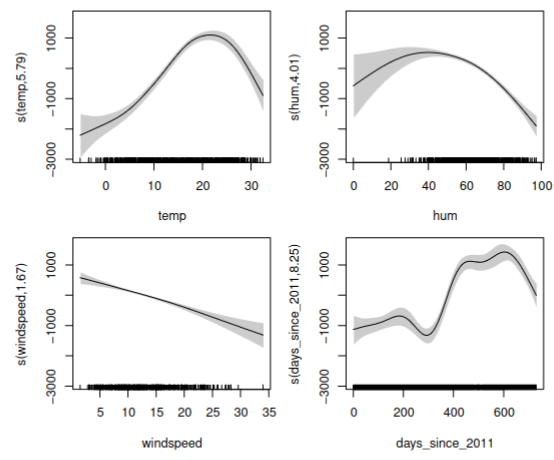
\includegraphics[width=0.2\textwidth]{figure/smooth_effects}
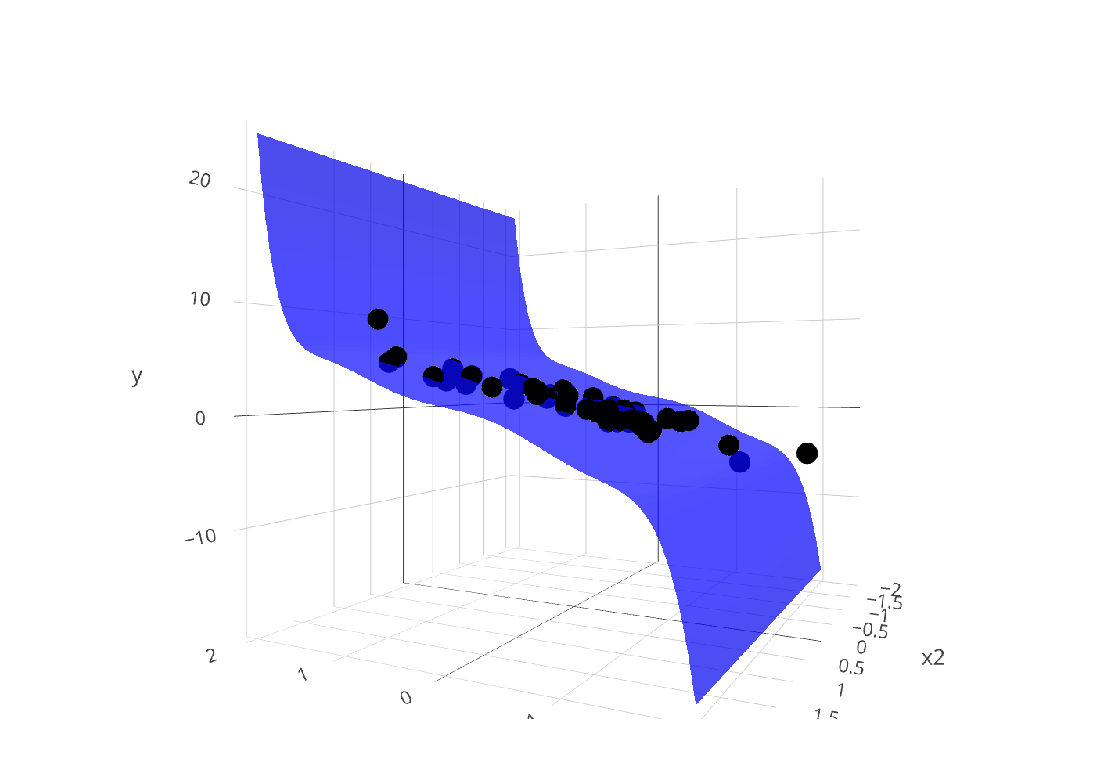
\includegraphics[width=0.2\textwidth]{figure/reg_poly_biv}

\textcolor{blue}{Figures still placeholders}

\framebreak

\highlight{Smooth functions}

\begin{itemize}
  \item Nonparametric/semiparametric/parametric approaches conceivable
  \item Frequently: express $f_j$ as weighted sum of \textbf{basis functions}
  $\rightsquigarrow$ model \textbf{linear} in weight coefficients again
  \begin{itemize}
      \item Use fixed basis of functions $b_1, \dots, b_K$ and estimate
      associated coefficients $\gamma_1, \dots, \gamma_K$ \\ $\rightsquigarrow$
      $f_j(x_j) = \sum_{k=1}^{K_j} \gamma_{j, k} b_k(x_j)$
      \item Popular types of basis functions
      \begin{itemize}
        \footnotesize
        \item Polynomial $\rightsquigarrow$ smoothing/TP-/B-\textbf{splines}
        \item Radial $\rightsquigarrow$ \textbf{Kriging}
        \item Trigonometric $\rightsquigarrow$ \textbf{Fourier/wavelet} forms
      \end{itemize}
    \end{itemize}
    \item Alternatives: \textbf{local regression (LOESS)}, other
    kernel-smoothing approaches, \dots
\end{itemize}

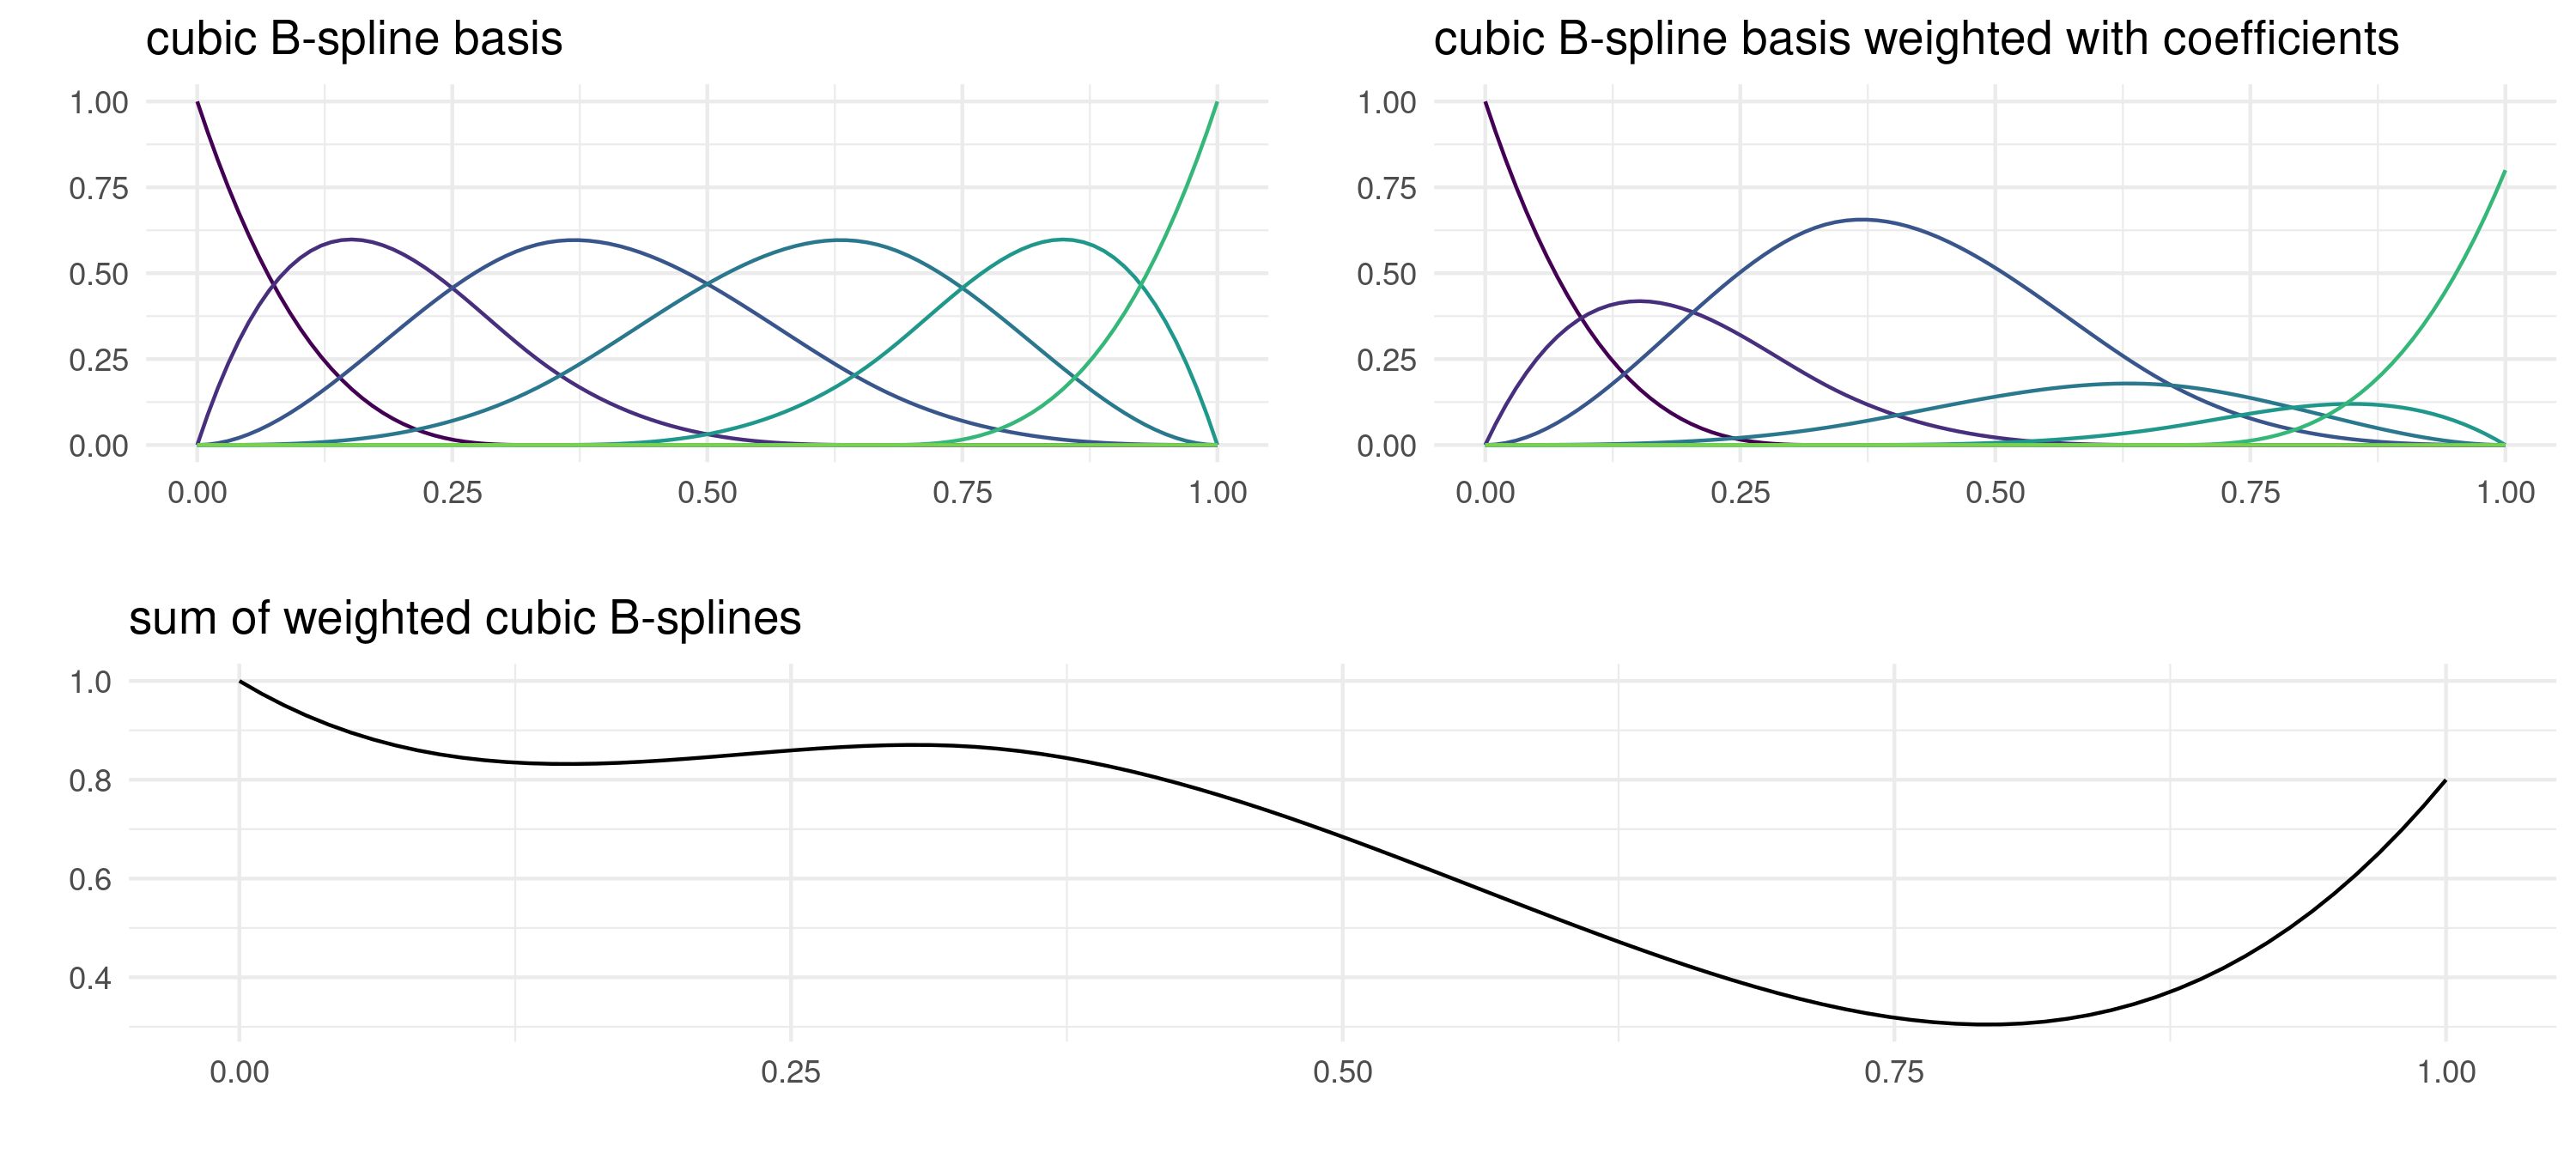
\includegraphics[width=0.4\textwidth]{figure/bspline-basis}

\end{vbframe}

% ------------------------------------------------------------------------------

\begin{frame}{Generalized Additive Models -- method summary}

\highlight{Regularization}
\begin{itemize}
    \item Smooth functions possibly very flexible $\rightsquigarrow$
    regularization vital to prevent overfitting
    \item Control \textbf{smoothness}
    \begin{itemize}
      \item \textbf{Basis-function approaches}: impose penalty on coefficients
      (e.g., magnitude or differences between coefficients of neighboring
      components) \& control associated hyperparameter
      \item \textbf{Local smoothers}: control width of smoothing window
      (larger $\rightsquigarrow$ smoother)
    \end{itemize}
\end{itemize}

\medskip
\textcolor{red}{TODO: pred surface for different degrees of smoothness}

\medskip

\highlight{Loss functions} ~~ Same as in GLM $\rightsquigarrow$ essentially:
use \textbf{negative log-likelihood}

\medskip

\highlight{Optimization}
\begin{itemize}
  \item \textbf{Coefficients} (of smooth + linear terms):
  penalized MLE, Bayesian inference
  \item \textbf{Smoothing hyperparameters}: typically, generalized
  cross-validation
\end{itemize}

\end{frame}

% ------------------------------------------------------------------------------

\begin{frame}{Generalized Additive Models -- implementation}

\highlight{Implementation}

\begin{itemize}
  \item \textbf{R:} \texttt{mlr3} learner \texttt{LearnerRegrGam},
    calling \texttt{mgcv::gam()}
  \begin{itemize}
      \item Smooth terms: \texttt{s(\dots, bs="<basis>")} or \texttt{te(\dots)}
      for multivariate (tensorproduct) effects
      \item Link functions: \texttt{family=$\{$Gamma, Binomial, \dots $\}$}
  \end{itemize}
    \item \textbf{Python}: \texttt{GLMGam} from package \texttt{statsmodels};
    package \texttt{pygam}
\end{itemize}

\medskip
\begin{columns}[onlytextwidth]
  \begin{column}{0.5\textwidth}
    \highlight{Advantages}

%    Strengths of GLMs, plus \dots
    \begin{itemize}
      \positem \textbf{Simple and fast} implementation
%      \positem \textbf{Analytical} solution for L2 loss
      %\positem \textbf{Cheap} computation
      \positem Applicable for any \textbf{dataset size}, as long as number of
      observations $\gg$ number of features
      \positem High \textbf{flexibility} via smooth effects
      \positem Easy to \textbf{combine} linear \& nonlinear effects
      \positem Intuitive \textbf{interpretability} via feature effects (though
      not quite as straightforward as in GLM)
      % \item fits \textbf{linearly} separable data sets very well
      \positem Statistical hypothesis \textbf{tests} for effects available
    \end{itemize}
  \end{column}

  \begin{column}{0.5\textwidth}
    \highlight{Disadvantages}

%    Shortcomings of GLMs, plus \dots
    \begin{itemize}
      \negitem \textbf{Sensitivity} w.r.t. outliers and noisy data
      \negitem Feature \textbf{interactions} must be handcrafted\\
      $\rightarrow$ practically infeasible for higher orders
      \negitem Harder to \textbf{optimize} than GLM
      \negitem Additional \textbf{hyperparameters} (type of smooth functions,
      smoothness degree, \dots)
    \end{itemize}
  \end{column}
\end{columns}

\end{frame}
